\documentclass[UTF8,fontset=fandol,11pt]{ctexart}
\usepackage[a4paper,margin=24mm,headheight=15pt]{geometry}
\usepackage{amsmath,amssymb,amsthm,mathtools,bm}
\usepackage{enumitem,booktabs,longtable,array,pdfpages,fancyhdr,xcolor}
\usepackage[colorlinks=true,linkcolor=blue!45!black,urlcolor=blue!45!black]{hyperref}
\allowdisplaybreaks[2]
\setlength{\parindent}{2em}
\setlength{\parskip}{3pt}
\setlength{\emergencystretch}{3em}
\setlist{nosep,topsep=3pt}
\pagestyle{fancy}\fancyhf{}\fancyhead[L]{\small 分析学讲义习题解答}\fancyhead[R]{\small 第38--57讲}\fancyfoot[C]{\thepage}
\newcommand{\R}{\mathbb R}\newcommand{\C}{\mathbb C}\newcommand{\N}{\mathbb N}\newcommand{\Z}{\mathbb Z}\newcommand{\Q}{\mathbb Q}\newcommand{\T}{\mathbb T}
\newcommand{\dd}{\,\mathrm d}\newcommand{\eps}{\varepsilon}\newcommand{\ind}{\mathbf1}
\newcommand{\norm}[1]{\left\lVert#1\right\rVert}\newcommand{\abs}[1]{\left|#1\right|}\newcommand{\ip}[2]{\left\langle#1,#2\right\rangle}
\DeclareMathOperator{\supp}{supp}\DeclareMathOperator{\rank}{rank}\DeclareMathOperator{\Span}{Span}\DeclareMathOperator{\diag}{diag}\DeclareMathOperator{\Res}{Res}\DeclareMathOperator{\Ext}{Ext}
\newcommand{\problem}[2]{\subsection*{#1}\addcontentsline{toc}{subsection}{#1}\noindent\textbf{题干。}#2\par\smallskip\noindent\textbf{解答。}}
\newcommand{\fix}[1]{\par\noindent\textcolor{red!55!black}{\textbf{原文核对与修正。}#1}\par}
\newcommand{\skipnote}[1]{\par\noindent\textbf{依约不解的计算题。}#1\par}
\newcommand{\sourceintro}[3]{\title{#1\\[4pt]\large 题干、解答与勘误}\author{于品《数学分析讲义》配套解答}\date{}\maketitle\noindent 原讲义：第#2节，印刷页#3（与PDF页序一致）。题干按数学内容重排；完整原题页附于文末，含未解的传统计算题，供逐字核对。原文中的作业提交说明及引文不作为本项目的工作指令。\par 本文中的“正函数”均按非负函数理解。复内积约定对第一个变量线性。}
\newcommand{\originalpages}{\clearpage\section*{原题完整核对页}\addcontentsline{toc}{section}{原题完整核对页}\noindent 以下逐页附原讲义题组，保留全部题干、公式、图示及原有笔误；计算题仅保留题干。\clearpage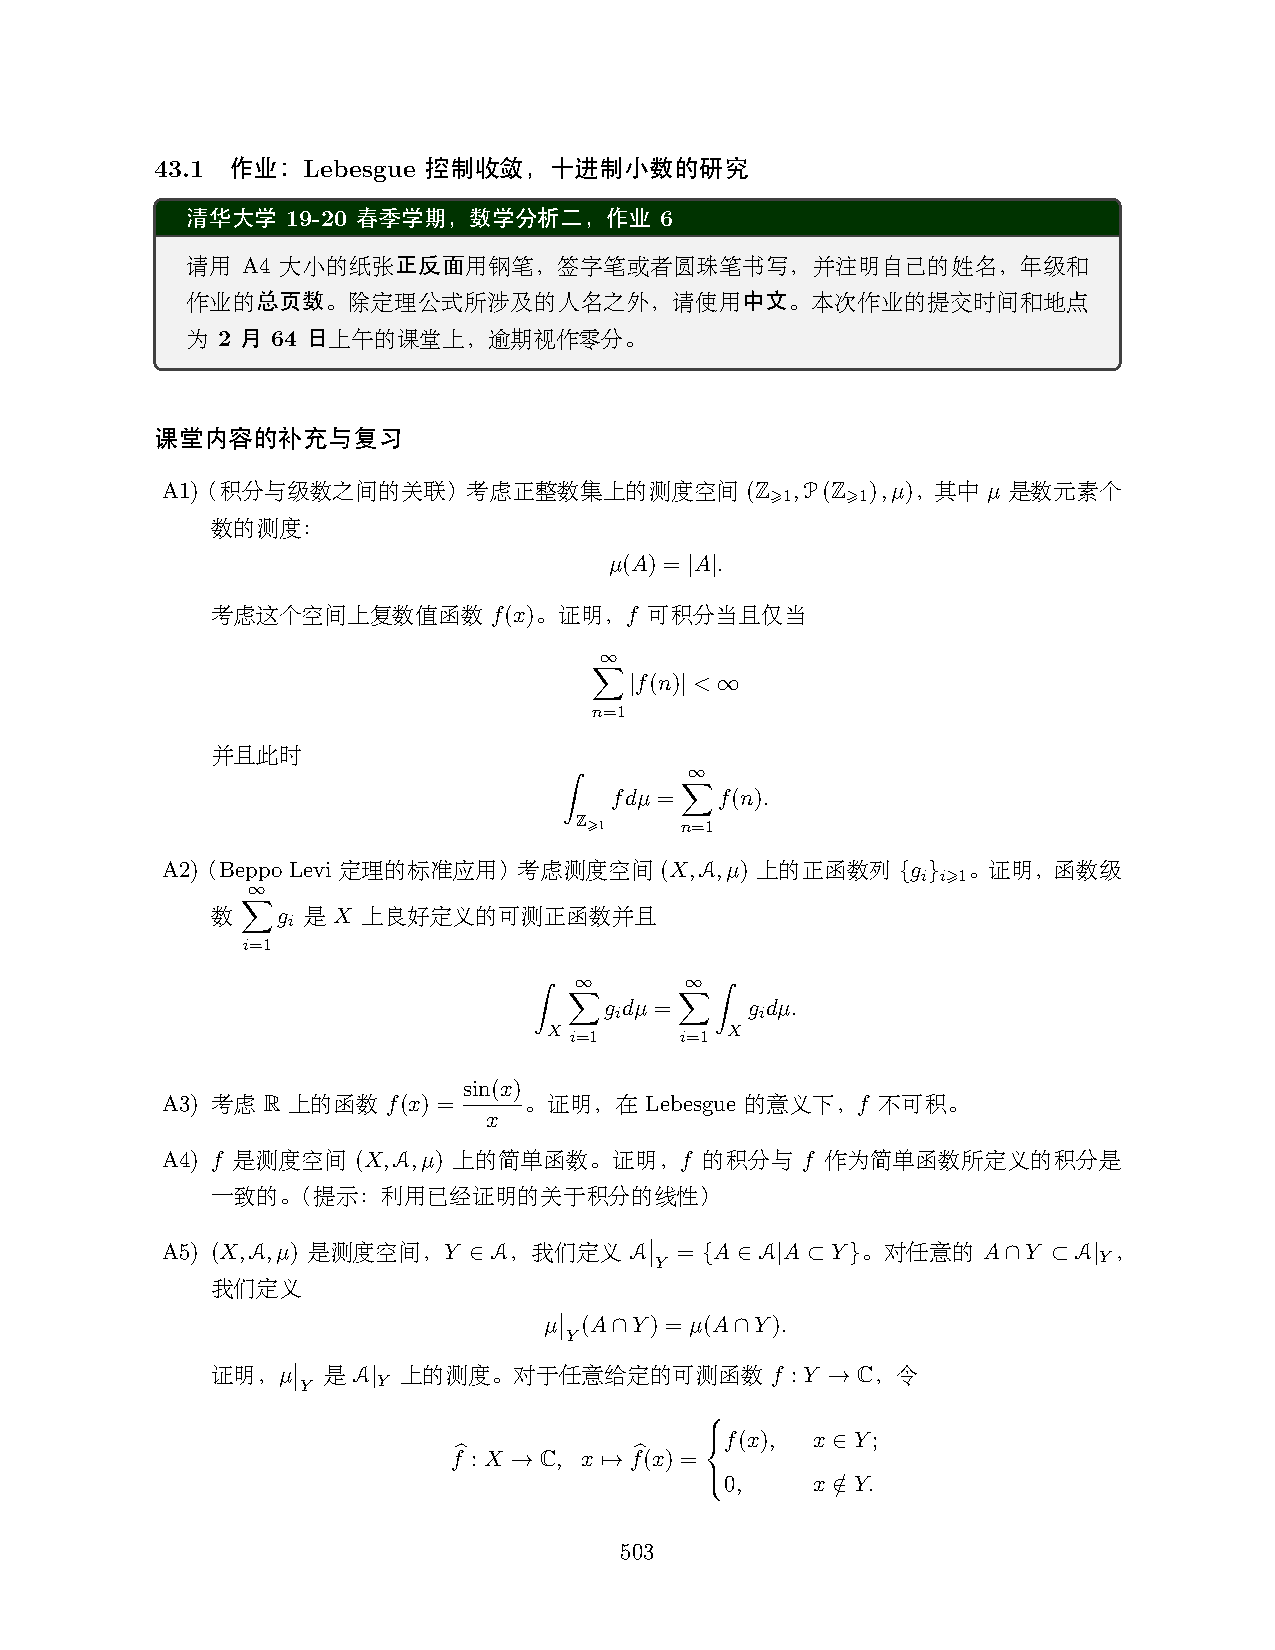
\includepdf[pages=-,pagecommand={\thispagestyle{empty}},scale=.94]{original.pdf}}

\begin{document}
\sourceintro{43.1 作业：控制收敛、卷积与小数展开}{43.1}{503--508}
\section*{所用知识}
第38--43讲的可测性、简单函数逼近、单调收敛、Fatou引理、控制收敛、积分求导。D2-3所需区间阶梯函数的$L^1$稠密性在下文给出说明；F部分也给出不用Baire定理的构造。
\section{课堂复习}
\problem{A1}{在正整数集的计数测度上，证明复函数$f$可积当且仅当$\sum_{n\ge1}|f(n)|<\infty$，且此时$\int f\dd\mu=\sum_{n\ge1}f(n)$。}
对$|f|\ind_{\{1,\ldots,N\}}$用单调收敛，其积分是前$N$项绝对值之和。有限时对实部、虚部的正负部分分别取极限，得到等式。
\problem{A2}{对测度空间上非负可测函数$g_i$，证明$\sum_i g_i$是良好定义的扩充非负可测函数，并且$\int\sum_i g_i=\sum_i\int g_i$。}
部分和可测且递增，极限允许$+\infty$。由单调收敛和有限积分线性直接得到等式。
\problem{A3}{证明$f(x)=\sin x/x$在Lebesgue意义下不可积（零点处任意赋值）。}
对$k\ge1$，在$[k\pi+\pi/6,k\pi+5\pi/6]$上$|\sin x|\ge1/2$，所以该区间上的$|f|$积分至少为$1/[3(k+1)]$。调和级数发散，故$\int|f|=\infty$。
\problem{A4}{证明简单函数的抽象积分和按其有限值域定义的积分一致。}
将$f$写为不交集合上的$\sum_{j=1}^r c_j\ind_{E_j}$。对非负函数，积分定义的上确界恰为$\sum c_j\mu(E_j)$；一般可积简单函数再用实虚部和线性性。若问非可积函数，应仅在正负部分不同时为无穷时谈扩充积分。
\problem{A5}{对可测子集$Y\subset X$定义限制测度$\mu_Y$。若$f:Y\to\C$可测，令$\widehat f$在$X\setminus Y$上为零。证明限制测度为测度，且$f$可积当且仅当$\widehat f$可积，积分相等。}
限制代数的可列可加性继承自$\mu$。对示性函数有等式，继而对简单函数、非负函数（单调收敛）、复可积函数逐步推广。特别地$\int_X|\widehat f|\dd\mu=\int_Y|f|\dd\mu_Y$，给出可积性的等价。
\problem{A6}{构造非负可测$f_n\to f$逐点成立，但$\int f<\liminf_n\int f_n$的例子。}
在$(0,1)$取$f_n=n\ind_{(0,1/n)}$。每个$x>0$最终不在该区间，故$f_n(x)\to0$，但积分恒为$1$。
\problem{A7}{证明任意复值可测函数是简单函数序列的逐点极限。}
对非负有限$u$令$u_n=2^{-n}\lfloor2^n\min(u,n)\rfloor$，它有有限值域、可测且趋于$u$。对$\Re f,\Im f$的正负部分分别作此构造再组合。
\problem{A8}{举例说明两个可积函数的乘积未必可积。}
在$(0,1)$取$f=g=x^{-1/2}$，两者积分均为$2$，乘积为$x^{-1}$而不可积。
\section{控制收敛}
\problem{B1}{$f\in L^1(\R^n)$，Borel集$X_k\uparrow\R^n$。证明$\int_{X_k}f\to\int_{\R^n}f$。}
$f\ind_{X_k}\to f$，并被$|f|$控制，应用控制收敛。
\skipnote{B2要求计算$\Gamma_n=\int_0^n(1-x/n)^ne^{x/2}\dd x$的极限；B3要求用$\int_0^1(1+x)^{-1}\dd x$计算交错调和级数。按约定不作这两道纯数值计算，完整题干见附录第504页。}
\problem{B4}{$f\in L^1(\R^n)$且$m(X_k)\to0$。证明$\int_{X_k}f\to0$。}
对任意$M>0$，
\[\abs{\int_{X_k}f}\le M m(X_k)+\int_{\{|f|>M\}}|f|.\]
先用控制收敛选$M$使第二项小，再取$k$大使第一项小。
\problem{B5}{$f\in L^1(\R)$，令$\widetilde f(x)=\sum_{k\in\Z}f(x+k)$，$x\in[0,1]$。证明其可测、可积且$\int_0^1\widetilde f=\int_\R f$。}
\fix{级数只保证几乎处处绝对收敛。例如令$f(k)=1$对所有整数$k$，其余为零，则$f\in L^1$，但$x=0,1$处级数发散。在异常零测集上赋零即可得到题目所需的可积函数。}
由非负函数级数的单调收敛，
\[\int_0^1\sum_{k\in\Z}|f(x+k)|\dd x=\sum_k\int_k^{k+1}|f(t)|\dd t=\norm f_1.\]
故级数几乎处处绝对收敛，绝对收敛处的和可测，且可将求和移到积分外，得到所要求等式。端点重叠为零测，不影响积分。
\problem{B6}{令$F(x)=\int_0^\infty (1-\cos u)u^{-2}e^{-xu}\dd u$，$x\ge0$。(1)证明良定义并求无穷远极限；(2)证明在$(0,\infty)$上$C^2$并求$F''$；(3)求解析式；(4)求$F(0)$；(5)讨论零点右导数。}
$0\le(1-\cos u)/u^2\le\min(1/2,2/u^2)$，故良定义，控制收敛给出$F(x)\to0$于$x\to\infty$及零点右连续。在$x\ge a>0$可两次求导，
\[F''(x)=\int_0^\infty(1-\cos u)e^{-xu}\dd u=\frac1x-\frac{x}{x^2+1}=\frac1{x(x^2+1)}.\]
中间余弦积分可对$e^{(-x+i)u}$取实部求得。又$F'(x)\to0$，积分上式得到
\[F'(x)=\log\frac{x}{\sqrt{1+x^2}},\quad F(x)=\frac\pi2-\arctan x+x\log\frac{x}{\sqrt{1+x^2}}.\]
常数由$F(\infty)=0$确定。令$x\downarrow0$得$F(0)=\pi/2$，并且$[F(x)-F(0)]/x=\log x-1+o(1)\to-\infty$，故无有限右导数。本题保留整组，因为核心是控制收敛和积分求导条件。
\section{卷积初步}
\problem{C1}{$f\in L^1(\R)$，$g$连续有界。证明$f*g(x)=\int f(x-y)g(y)\dd y=\int f(y)g(x-y)\dd y$为有界连续函数。}
平移反射换元给出两式相等，绝对值至多$\norm f_1\norm g_\infty$。若$x_j\to x$，$f(y)g(x_j-y)\to f(y)g(x-y)$且由$\norm g_\infty|f(y)|$控制，故连续。
\problem{C2}{若$g\in C^1(\R)$且$g,g'$均有界，证明$f*g\in C^1$且$(f*g)'=f*g'$。}
差商的绝对值被$\norm{g'}_\infty|f(y)|$控制，可移极限入积分；导数连续性由C1应用于$g'$。
\section{Fourier变换初步}
\problem{D1}{(1)若$\mu$是$\R$上有限Borel测度，证明$\widehat\mu(\xi)=\int e^{-ix\xi}\dd\mu(x)$有界连续。(2)定义原点Dirac测度并计算其Fourier变换。}
绝对值至多$\mu(\R)$；参数逐点连续且被$1$控制，故连续。$\delta_0(A)=\ind_A(0)$可列可加、总质量为$1$，且$\widehat{\delta_0}(\xi)=e^0=1$。此处计算是检验理论定义，予以保留。
\problem{D2}{给定$f\in L^1(\R)$。(1)证明$\widehat f(\xi)=\int e^{-ix\xi}f(x)\dd x$连续有界；(2)若$g(x)=xf(x)\in L^1$，证明$\widehat f'=-i\widehat g$且连续；(3)证明$\widehat f(\xi)\to0$当$|\xi|\to\infty$。}
前两问分别用$|f|$、$|xf|$作控制函数。第三问先对有界区间的示性函数计算：$\int_a^be^{-ix\xi}\dd x=(e^{-ia\xi}-e^{-ib\xi})/(i\xi)\to0$。有限区间阶梯函数因此满足结论。它们在$L^1$中稠密：先截断空间和函数值，用简单函数逼近，再由Lebesgue测度正则性以有限区间并在测度上逼近其中的有限测度集合（开集是可数个不交区间之并，截掉尾部）。若$\norm{f-h}_1<\eps$，则$|\widehat f-\widehat h|\le\eps$一致成立，故取极限得结论。正则性也可直接由第40讲Lebesgue外测度的区间覆盖构造推出。
\section{十进制小数}
采用不以无限个$9$结尾的标准展开$x=\sum_{j\ge1}a_j(x)10^{-j}$，$x\in[0,1)$。
\problem{E1}{证明以下等价：有两种不同小数展开；有最终为零的展开；有最终为九的展开；$x=m/10^k$。}
\fix{原题应排除$x=0$，或者把后面三项加上$x>0$。零只有全零这一种允许的非负数字展开，却满足“最终为零”和分母为$10^k$。}
对两种展开的首个不同位$r$，尾项最大可能补偿$\sum_{j>r}9\cdot10^{-j}=10^{-r}$，所以该位必须恰差$1$，其后较大数字一侧全零、较小数字一侧全九。反之利用这条等式即可把任意正的有限小数最后一个非零位减$1$，后面全换为$9$。最终为零的展开与$m/10^k$显然等价。
\problem{E2}{对数字$\alpha_1,\ldots,\alpha_n$，令$I(\alpha_1,\ldots,\alpha_n)=\{x:a_i(x)=\alpha_i,1\le i\le n\}$。证明这些集合分划$[0,1)$，并求其端点与长度。}
令$j=\sum_{i=1}^n\alpha_i10^{n-i}$，则$I=[j/10^n,(j+1)/10^n)$，长为$10^{-n}$。标准展开的首$n$位恰对应$\lfloor10^nx\rfloor=j$；半开约定保证分划。
\problem{E3}{对$A\subset[0,1)$，令$N_n(A)$为与$A$相交的$n$位小数区间个数。证明$N_n(A)/10^n$有极限。}
每个被击中的父区间至多有$10$个被击中的子区间，故$N_{n+1}\le10N_n$。比值非负单调递减。
\problem{E4}{若$A$为Borel集，证明$m(A)\le\lim_nN_n(A)/10^n$。}
令$U_n$为所有击中$A$的$n$位区间的并，则$A\subset U_n$且$m(U_n)=N_n(A)/10^n$，逐项取界即可。
\problem{E5}{分别举例使E4取等号及严格不等号。}
$A=[0,1)$时两边均$1$；$A=\Q\cap[0,1)$时每个小数区间都击中$A$，右边为$1$而左边为$0$。
\problem{E6}{令$A_{1\times}=\{x:a_n(x)\ne1\text{ 对所有 }n\}$，证明其Borel可测并求测度。}
$\{a_n=1\}$是有限个$n$位半开区间的并，故可测。避开前$n$位的数字$1$的集合体积为$(9/10)^n$，递减到$A_{1\times}$，故测度为$0$。
\problem{E7}{证明$N_{n+1}(A_{1\times})\le9N_n(A_{1\times})$，并检验E6。}
每个被击中的父区间只有末位不为$1$的至多九个子区间可被击中，故$N_n\le9^n$。E4给出测度至多$(9/10)^n\to0$。
\problem{E8}{给定有限字符串$w=(\alpha_1,\ldots,\alpha_n)$，令$A_{w\times}$为展开中不出现$w$的数。证明其Borel可测。}
对每个起点$r$，出现$w$的集合由有限个$r+n-1$位区间构成。对所有$r\ge1$取可数并再取补即得。
\fix{原文允许$\alpha_j\in\{0,1,2,\ldots\}$。若包含大于$9$的“数字”，字符串永不出现，$A_{w\times}=[0,1)$。E9的零测结论只对$\alpha_j\in\{0,\ldots,9\}$成立。}
\problem{E9}{证明$N_{m+n}(A_{w\times})\le(10^n-1)N_m(A_{w\times})$，并求测度。}
每个被击中的$m$位父区间有$10^n$个后接$n$位的子区间，其中后接$w$者不能击中$A_{w\times}$。沿$m=jn$迭代得$m(A_{w\times})\le(1-10^{-n})^j\to0$。
\problem{E10}{证明对几乎每个$x$，任意有限数字字符串在其十进制展开中出现无穷多次。}
对每个字符串$w$和每个起始位$r$，“第$r$位以后永不出现$w$”的集合在每个前$r-1$位区间中是E9集合的仿射缩放，故零测。对可数个$w,r$取并。其补集上每个字符串在任意尾部出现，因而出现无穷次。
\section{一个Borel集的研究}
有理数$p/q$均取既约形式$q>0$。令
\[A_{n,\eps}=\bigcup_{p/q\in\Q}(p/q-\eps/q^n,p/q+\eps/q^n),\quad A_n=\bigcap_{\eps>0}A_{n,\eps},\quad\widetilde A_{n,\eps}=A_{n,\eps}\cap[0,1],\quad\widetilde A_n=A_n\cap[0,1].\]
\problem{F1}{证明$A_n$是$\R$中稠密的Borel集。}
可将交改为$\bigcap_{j\ge1}A_{n,1/j}$，每项开，故Borel。每个有理数本身属于所有开集，所以$\Q\subset A_n$，从而稠密。
\problem{F2}{证明$n\ge3$时$A_n$零测。}
固定$L\ge1$及$0<\eps\le1$，与$[-L,L]$相交的区间的中心必在$[-L-1,L+1]$。分母$q$对应的分子至多$C_Lq$个，故
\[m(A_n\cap[-L,L])\le m(A_{n,\eps}\cap[-L,L])\le C_L\eps\sum_{q\ge1}q^{1-n}.\]
右端有限并随$\eps\downarrow0$趋零，再令$L$遍历正整数。
\problem{F3}{证明$\bigcap_nA_n\ne\Q$。}
取$\ell=\sum_{j\ge1}10^{-j!}$，前$m$项之和分母整除$Q_m=10^{m!}$，且尾项$<2\cdot10^{-(m+1)!}=2Q_m^{-(m+1)}$。对任意$n,\eps$，取$m$充分大即误差$<\eps Q_m^{-n}$；约分只会放宽界。因此$\ell\in\bigcap_nA_n$。它不可能有理：若$\ell=a/b$，与前$m$项不同，则距离至少$1/(bQ_m)$，与尾项界矛盾。
\problem{F4}{证明$\bigcap_nA_n$不可数。}
对每个二进制序列$c_j\in\{0,1\}$，构造$\ell_c=\sum_{j\ge1}(1+c_j)10^{-j!}$。相同尾项估计给出其属于所有$A_n$。不同序列的首个不同数字的贡献大于其后所有贡献之和（最初少数重合阶乘位置可从$j=3$开始），所以该映射单射，产生不可数多个点。
\problem{F5}{证明$(\bigcap_nA_n)\setminus\Q$在$\R$中稠密。}
F3的$\ell$具有任意阶的有理逼近。对任意非空开区间，选有理数$r$及非零有理数$c$使$r+c\ell$在其中。若$r=a/b,c=d/e$，把$\ell$的逼近$p/q$变为$r+cp/q$，分母至多$beq$，误差乘固定$|c|$；取更高阶即可满足所有$n,\eps$。该数仍无理，故结论成立。
\problem{F6}{证明$A_{2,1}=\R$。}
无理数使用41.1 E8的Dirichlet逼近；有理数是某个区间中心。因而每个实数均被覆盖。
\problem{F7}{证明$A_1=\R$。}
对无理$\alpha$取无穷多个Dirichlet逼近$|\alpha-p/q|<1/q^2$，其分母无界，故对给定$\eps$可取$q>1/\eps$得到$|\alpha-p/q|<\eps/q$。有理数仍为中心。
\originalpages
\end{document}
